\documentclass[compress,aspectratio=169]{beamer}

\usetheme{metropolis}
\setbeamersize{text margin left=.5cm,text margin right=.5cm}
%  \setbeamertemplate{navigation symbols}{} % suppress nav bar
%  \setbeamercovered{transparent}

\usefonttheme{professionalfonts}
\usepackage{tikz}
\usepackage{amsmath}
\usepackage{mathpazo}
\usepackage{xcolor,colortbl}
\usepackage{siunitx}
\usepackage{bm}

\setmonofont{Ubuntu Mono}
\setlength{\parskip}{0pt}
\renewcommand{\baselinestretch}{1}

\sisetup{
  detect-all,
  number-math-rm=\mathnormal,
  per-mode=symbol
}

\title{Topic 21: Light Waves and Optics}
\subtitle{Advanced Placement Physics}
\author[TML]{Dr.\ Timothy Leung}
\institute{Olympiads School\\Toronto, Ontario, Canada}
\date{April 2020}

\newcommand{\pic}[2]{\includegraphics[width=#1\textwidth]{#2}}
\newcommand{\mb}[1]{\mathbf{#1}}
\newcommand{\eq}[2]{\vspace{#1}{\LARGE\begin{displaymath}#2\end{displaymath}}}

\begin{document}

\begin{frame}
  \maketitle
\end{frame}


%\begin{frame}{In This Class}
%  In this unit, we will be discussing some important properties of light:
%  \begin{itemize}
%  \item Light waves passing through a medium
%    \begin{itemize}
%    \item Reflection
%    \item Refraction
%    \item Dispersion
%    \end{itemize}
%  \item Light waves passing through an opening
%    \begin{itemize}
%    \item Diffraction
%    \item Interference
%    \item Optical resolution
%    \end{itemize}
%  \item The nature of light? (What kind of wave is light?)
%    \begin{itemize}
%    \item Electromagnetic waves
%    \item Polarization of light
%    \end{itemize}
%  \item Geometric Optics
%    \begin{itemize}
%    \item Mirrors
%    \item Thin lens equation
%    \end{itemize}
%  \end{itemize}
%  Some of the topics that we are discussing are reviews\ldots but with new
%  insights and more information.
%\end{frame}



\section{Huygens}

\begin{frame}{Huygens' Principle}
  In the 1600's there were two competing theories of light\ldots
  \begin{itemize}
  \item Some, including Issac Newton, believed that  light is a particle
  \item Others, including Christiaan Huygen (Dutch) and Augustin-Jean Fresnel
    (French), believed that light is a wave
  \end{itemize}
  \vspace{0.4in}

  Huygen's Princple: all waves are in fact an infinite series of circular
  wavelets
\end{frame}


\section{Reflection}

\begin{frame}{Reflection of Light}
  In the \textbf{law of reflection}, the incident ray, the reflected ray, and
  the normal to the surface of the mirror all lie in the same plane, and the
  angle of reflection is equal to the angle of incidence
  \begin{center}
    \pic{.7}{graphics/Types-of-reflection.png}
  \end{center}
\end{frame}


\begin{frame}{Specular Reflection Example}
  \begin{center}
    \pic{.55}{graphics/Lake-reflection.jpg}
  \end{center}
  This photo of Lake Matheson shows specular reflection in the water of the
  lake with reflected images of Aoraki/Mt Cook (left) and Mt Tasman (right).
  The very still lake water provides a perfectly smooth surface for this to
  occur.
\end{frame}



\section{Refraction}

\begin{frame}{Refraction of Light Through a Medium}
  \begin{columns}
    \column{0.4\textwidth}
    \begin{itemize}
    \item When a wave enters another medium, the wave speed changes
    \item When entering at an angle, the change of speed causes the wave to
      change direction (e.g.\ from air to water, air to glass, glass to air etc)
    \item The amount of bending depends on the
      \textbf{indices of refraction of the two media}
    \item Responsible for \textbf{image formation} by lenses and the eye
    \end{itemize}
    \column{0.6\textwidth}
    \pic{1}{graphics/negative_refraction.jpg}
  \end{columns}
\end{frame}



\begin{frame}{Refraction of Light Through a Medium}
  Light entering from one medium to another at an angle results in refraction
  In the diagram, light could be going in either direction, from top to bottom
  ($n_1$ to $n_2$) or from bottom to top ($n_2$ to $n_1$)
  \begin{center}
    \vspace{-.2in}
    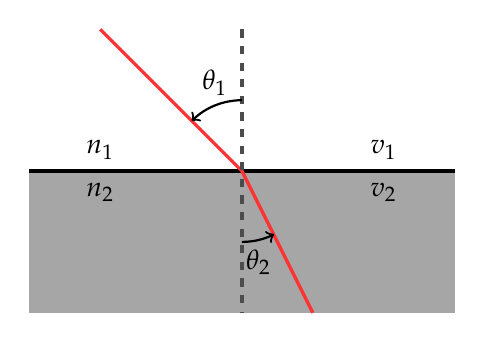
\begin{tikzpicture}[scale=.9]
      \fill[gray!70](-3,-2) rectangle (3,0);
      \draw[very thick](-3,0)--(3,0);
      \draw[red!80,very thick](-2,2)--(0,0)--(1,-2);
      \draw[dashed,black!70,very thick](0,2)--(0,-2);
      \draw[->,thick](0,1) arc(90:135:1) node[midway,above]{$\theta_1$};
      \draw[->,thick](0,-1)arc(270:297:1) node[midway,below]{$\theta_2$};
      \node at (-2,.3) {$n_1$};
      \node at (-2,-.3){$n_2$};
      \node at (2,.3) {$v_1$};
      \node at (2,-.3){$v_2$};
    \end{tikzpicture}
  \end{center}
  \textbf{Snell's law} relates the refractive indices $n$ of the two media
  to the directions of propagation in terms of the angles $\theta$ to the
  normal

  \eq{-.2in}{
    \boxed{n_1\sin\theta_1=n_2\sin\theta_2}
  }
\end{frame}



\begin{frame}{Refraction and Huygens Principle}
  \begin{columns}
    \column{.5\textwidth}
    \pic{1}{graphics/huygen.png}
    
    \column{.5\textwidth}
    We can explain the refraction phenomenon using Huygens' Principle
  \end{columns}
\end{frame}



\begin{frame}{Index of Refraction}
  \textbf{Index of refraction} ($n$) (or \textbf{refractive index}, or just
  \textbf{index}) is the ratio of the speed of light in a vacuum ($c_0$) to the
  speed of light in the medium ($c$):

  \eq{-.2in}{
    \boxed{n=\frac{c_0}{c}=\frac{\lambda_\mathrm{vacuum}}{\lambda}}
  }

  When light enters a second medium, the \emph{frequency} remains unchanged but
  since the speed changes, the \emph{wavelength} also changes:
    
  \eq{-.2in}{
    \boxed{\frac{n_1}{n_2}=\frac{\lambda_2}{\lambda_1}}
  }

  You can work this out using the univesal wave equation: $v=f\lambda$
\end{frame}


\begin{frame}{Index of Refraction of Common Materials}
  \begin{center}
    \begin{tabular}{c|c||c|c}
      \rowcolor{pink}
      \textbf{Material} & $\bm{n}$ & \textbf{Material} & $\bm{n}$\\ \hline
      Vacuum           & 1        & Ethanol     & 1.362 \\
      Air              & 1.000277 & Glycerine   & 1.473 \\
      Water at \SI{20}{\celsius} & 1.33 & Ice         & 1.31 \\
      Carbon disulfide & 1.63     & Polystyrene & 1.59 \\
      Methylene iodide & 1.74     & Crown glass & 1.50-1.62\\
      Diamond          & 2.417    & Flint glass & 1.57-1.75\\
    \end{tabular}
  \end{center}
  The values given are \emph{approximate} and do not account for the small
  variation of index with light wavelength. That's called \textbf{dispersion}.
\end{frame}



\begin{frame}{Total Internal Reflection}
  \textbf{Total internal reflection} (``TIR'') occurs when light enters from a
  medium with high index to another medium with low index (i.e.\ $n_1>n_2$).
  Snell's law still holds, but something weird can happen:
  \begin{center}
    \pic{.6}{graphics/660px-RefractionReflextion.png}
  \end{center}
  Critical angle $\theta_c$ for water-air interface is \ang{48.6}. TIR occurs
  when the incident angle is greater $\theta_1>\theta_c$.
\end{frame}



\section{Dispersion}

\begin{frame}{Color of Light and Wavelength}
  Human eyes perceive different frequencies of light as different colors. The
  visible spectrum of light:
  \begin{center}
    \pic{.4}{graphics/visiblespectrum.png}
  \end{center}
  \begin{itemize}
  \item The \emph{color} of the light depends on its frequency (\& wavelength
    when it's in a vacuum)
  \item \emph{White light} is light that contains waves in all frequencies.
  \end{itemize}
\end{frame}



\begin{frame}{Dispersion of Light Through Refraction}
  \begin{columns}
    \column{.4\textwidth}
    \pic{1}{graphics/white-light-split-into-colours-by-a-prism-pasieka.jpg}

    \column{.55\textwidth}
    \begin{itemize}
    \item When white light passes through a prism it is separated into
      different colors (spectrum) through refraction.
    \item This is because the index of refraction $n$ is slightly different for
      different wavelengths
    \item Otherwise, we will never see a rainbow
    \end{itemize}
  \end{columns}
\end{frame}



\begin{frame}{Wavelength Dependency of Index of Refraction}
  \begin{center}
    \pic{.5}{graphics/Dispersion-curve.png}
  \end{center}
\end{frame}



\section{Interference}

\begin{frame}{Thomas Young's Double-Slit Experiment}
  \begin{columns}
    \column{.45\textwidth}
    \pic{1}{graphics/double-slit1.png}
    
    \column{.52\textwidth}
    \begin{itemize}
    \item\textbf{Monochromatic light} light with a single color (frequency);
      the light source can be a laser, LED , or gas lamp (most likely what Young
      used)
    \item\textbf{Slit:} an opening; also called an \textbf{aperture}
    \item The \textbf{screen} far away from the slits is also called the
      \textbf{projection}
    \end{itemize}
  \end{columns}

  \vspace{.15in}Double-slit experiment showed that light causes interference,
  just like any other wave
\end{frame}

\begin{frame}{Thomas Young's Double-Slit Experiment}
  \begin{columns}
    \column{.28\textwidth}
    \pic{1.15}{graphics/path1.png}
    
    \column{.72\textwidth}
    \begin{itemize}
    \item At \textbf{A}, the path from slits $S_1$ and $S_2$ are the same,
      therefore we have \textbf{constructive interference} and the projection
      is bright
    \item At \textbf{B}, the path from $S_1$ and $S_2$ are diffed by half a
      wavelength, and therefore there is \textbf{destructive interference} and
      the projection is dark
    \item At \textbf{C}, the path from $S_1$ and $S_2$ are diffed by one
      wavelength, and therefore there is \textbf{constructive interference}
      again, and again, the projection is bright
    \end{itemize}
  \end{columns}
\end{frame}



\begin{frame}{Interference Pattern: Bright and Dark Fringes}
  \begin{center}
    \pic{.4}{graphics/fringes1.png}
  \end{center}
  The ``bright fringes'' are from constructive interference; the ``dark
  fringes'' are from destructive interference.
\end{frame}



\begin{frame}{Let's Work This Out!}
  \begin{columns}
    \column{0.5\textwidth}
    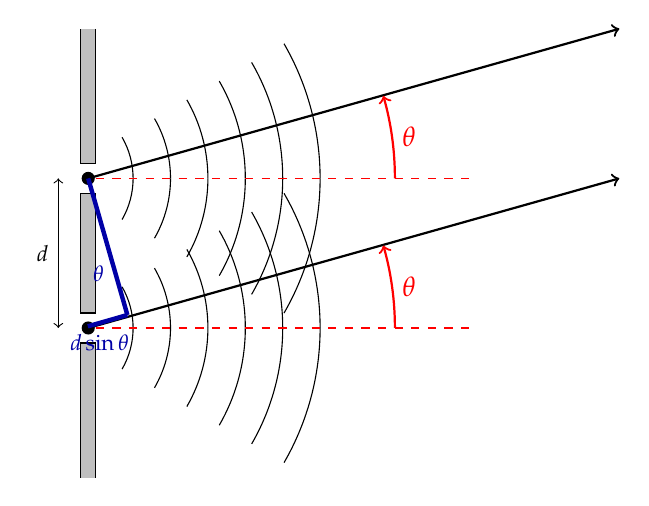
\begin{tikzpicture}[scale=0.95]
      \draw[fill=gray!50](0,3)--(0,1.2)--(-0.2,1.2)--(-0.2,3);
      \draw[fill=gray!50](0,0.8)--(0,-0.8)--(-0.2,-0.8)--(-0.2,0.8)--cycle;
      \draw[fill=gray!50](0,-3)--(0,-1.2)--(-0.2,-1.2)--(-0.2,-3);
      \draw[<->](-0.5,-1)--(-0.5,1) node[midway,left]{\footnotesize $d$};
      
      \draw[fill=black](-0.1,1) circle(0.08);
      \draw[fill=black](-0.1,-1)circle(0.08);
      \foreach \x in {0.5,1,...,3} {
        \pgfmathsetmacro\xx{\x+0.6};
        \draw(\x,1) arc(0:30:\xx); \draw(\x,1) arc(0:-30:\xx);
        \draw(\x,-1)arc(0:30:\xx); \draw(\x,-1)arc(0:-30:\xx);
      }

      \draw[thick,->](-0.1,1)--(7,3);
      \draw[thick,->](-0.1,-1)--(7,1);

      \draw[red,thick,->](4,1) arc(0:16:4) node[midway,right]{$\theta$};
      \draw[red,thick,->](4,-1)arc(0:16:4) node[midway,right]{$\theta$};
      \draw[red,dashed](0,1)--(5,1);
      \draw[red,dashed](0,-1)--(5,-1);

      \begin{scope}[rotate around={16:(-0.1,1)}]
        \draw[blue!65!black,ultra thick](-0.1,1)--(-0.1,-0.9)
        node[pos=0.7,left]{\footnotesize $\theta$};
        \draw[blue!65!black,ultra thick](-0.1,-0.9)--(-0.65,-0.9)
        node[pos=0.7,below]{\footnotesize $d\sin\theta$};
      \end{scope}

    \end{tikzpicture}
    \column{0.47\textwidth}
    \begin{itemize}
    \item We have two slits at distance $d$ apart, emitting \emph{coherent}
      light
    \item Huygens' Principle: light passing through the slits become point
      sources
    \item Assume that the projection (screen) is far enough from the slits
      that we can treat the two beams of light from the slits as being parallel
    \item Using basic geometry, we can see that the path difference from the
      two slit to the projection is $d\sin\theta$
    \end{itemize}      
  \end{columns}
\end{frame}



\begin{frame}{Contructive Interference with Double-Slits}
  A bright fringe (constructive interference) happens if the path difference
  ($d\sin\theta$) is an integer ($n$) multiple of wavelength ($\lambda$):
  
  \eq{-.2in}{
    \boxed{n\lambda = d\sin\theta_n}
  } 

  \vspace{-.2in}where $n=0,1,2,3\ldots$
  \begin{center}
    \begin{tabular}{l|c|c}
      \rowcolor{pink}
      \textbf{Quantity} & \textbf{Symbol} & \textbf{SI Unit} \\ \hline
      Integer number of full wavelengths & $n$       & (none)\\
      Wavelength of light                & $\lambda$ & \si{\metre}\\
      Distance between slits             & $d$       & \si{\metre}\\
      Deflection angle                   & $\theta$  & (unit less)
    \end{tabular}
  \end{center}
  The last fringe $n_\mathrm{max}$ can be found by setting $\sin\theta=1$.
  Therefore the total nubmer of bright fringes $N$:

  \eq{-.3in}{
    N=2n_\mathrm{max}+1
  }
\end{frame}


\begin{frame}{Destructive Interference with Double-Slits}
  Conversely, dark fringes (destructive interference) occurs when the path
  difference ($d\sin\theta$) is an half-number ($n+\frac12$) multiple of
  wavelength ($\lambda$):
  
  \eq{-.2in}{
    \boxed{\left(n+\frac{1}{2}\right)\lambda = d\sin\theta_n}
  }
  
  where $n=0,1,2,3\ldots$. Again, the last dark fringe $n_\mathrm{max}$ can be
  found by setting $\sin\theta=1$, and the total nubmer of dark fringes $N$:

  \eq{-.25in}{
    N=2n_\mathrm{max}
  }
\end{frame}



%\begin{frame}
%  \frametitle{Double-Slit Interference}
%  \begin{center}
%    \pic{0.65}{graphics/path-difference.png}
%  \end{center}
%\end{frame}


\begin{frame}{Approximation of The Wavelength of Light}
  We can actually estimate the wavelength of light based on the distances
  between bright fringes, by applying the \textbf{small-angle approximation}:
  
  \eq{-.3in}{
    \theta\approx\tan\theta\approx\sin\theta
  }
  
  \vspace{-.15in}We can already relate the distance from slits to the screen
  ($x$), and the distance of the $n$-th bright fringe from the centre ($y_n$)
  to $\theta_n$. Applying the approximation, we have:

  \eq{-.2in}{
    \tan\theta_n=\frac{y_n}{x}\approx\sin\theta_n
  }

  Substitute this approximation into the constructive interference equation:

  \eq{-.2in}{
    n\lambda\approx\frac{y_nd}{x}
    \quad\longrightarrow\quad
    \boxed{\lambda\approx\frac{\Delta y d}{x}}
  }
\end{frame}



\begin{frame}{Approximation of The Wavelength of Light}
  This equation applies equally to dark fringes (nodal lines) as well as bright
  fringes.
  
  \eq{-.2in}{
    \boxed{\lambda\approx\frac{\Delta y d}{x}}
  }
  \begin{center}
    \begin{tabular}{l|c|c}
      \rowcolor{pink}
      \textbf{Quantity} & \textbf{Symbol} & \textbf{SI Unit} \\ \hline
      Wavelength                     & $\lambda$  & \si{\metre} \\
      Distance between fringes       & $\Delta y$ & \si{\metre} \\
      Distance between slits         & $d$        & \si{\metre} \\
      Distance from source to screen & $x$        & \si{\metre}
    \end{tabular}
  \end{center}
  Since the approximation is based on small angles, we must apply this equation
  to where $\Delta y$ close to the centre, where light from both slits are
  deflected by a small angle.
\end{frame}


\begin{frame}
  \frametitle{Important Notes}
  \begin{itemize}
  \item We have applied the double-slit problem specifically to light, but it
    can be applied to any mechanical wave (e.g.\ sound waves, ocean waves) as
    well
  \item The sources don't actually need to be slits; any point source will do
  \item The projection/screen doesn't need to be a real screen either; it just
    has to be a line where wave intensity can be measured
  \end{itemize}
\end{frame}



\section{Diffraction}

\begin{frame}{Diffraction of Waves}
  When a wave goes through an small opening, it \textbf{diffracts}. This happens
  with sound waves, ocean waves\ldots and light.
  \begin{center}
    \pic{.55}{graphics/alexandria.jpg}
  \end{center}
  The photo is from the Port of Alexandria in Egypt. The shape of the entire
  harbor is created because of diffraction of ocean wave.
\end{frame}



\begin{frame}{Diffraction of Waves}
  \begin{center}
    \pic{.6}{graphics/diffraction1.jpg}
  \end{center}
  The smaller the opening (compared to the wavelength of the incoming wave)
  the greater the diffraction effects.
\end{frame}


\begin{frame}{Equations for Diffraction}
  \begin{columns}
    \column{.4\textwidth}
    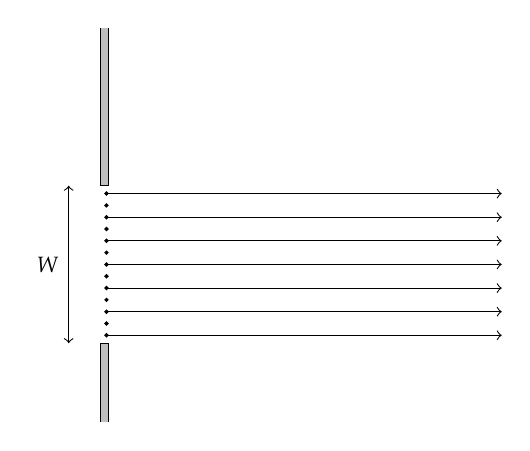
\begin{tikzpicture}
      \draw[fill=gray!50](0,3)--(0,1)--(-0.1,1)--(-0.1,3);
      \draw[fill=gray!50](0,-2)--(0,-1)--(-0.1,-1)--(-0.1,-2);
      \draw[<->](-0.5,-1)--(-0.5,1) node[midway,left]{\footnotesize $W$};
      \foreach \y in {1,...,13} {
        \pgfmathsetmacro\yy{1.05-0.15*\y};
        \draw[fill=black](-0.02,\yy) circle(0.02);
      }

      \foreach \y in {1,3,...,13} {
        \pgfmathsetmacro\yy{1.05-0.15*\y};
        \draw[->](-0.02,\yy)--(5,\yy);
      }
    \end{tikzpicture}
    
    \column{.57\textwidth}
    \begin{itemize}
    \item Similar to the double-slit problem, we apply Huygens' Principle
      again
    \item This time we treat the slit as wide enough that there is a series
      (an infinite series, actually) of point waves at the slit
    \item We can easily see that the light from the wavelet that travel
      perpendicular to the slit (aperture) will not interfere with one another
    \item i.e.\ a bright fringe at the middle.
      \textbf{This is called the central maximum.}
    \end{itemize}
  \end{columns}
\end{frame}




\begin{frame}{At Some Other Angle $\theta$}
  \begin{columns}
    \column{0.4\textwidth}
    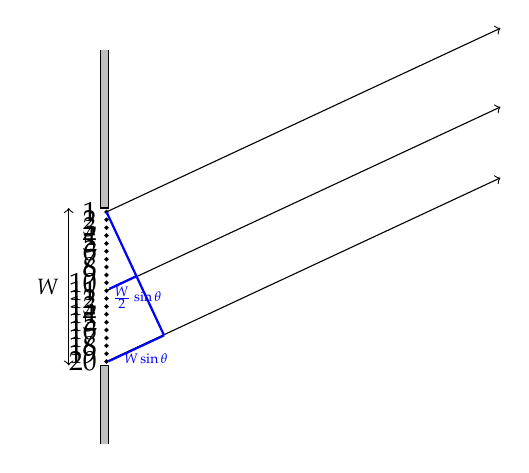
\begin{tikzpicture} %[scale=0.95]
      \draw[fill=gray!50](0,3)--(0,1)--(-0.1,1)--(-0.1,3);
      \draw[fill=gray!50](0,-2)--(0,-1)--(-0.1,-1)--(-0.1,-2);
      \draw[<->](-0.5,-1)--(-0.5,1) node[midway,left]{\footnotesize $W$};
      \foreach \y in {1,...,20} {
        \pgfmathsetmacro\yy{1.05-0.1*\y};
        \draw[fill=black](-0.02,\yy) circle(0.02) node[left]{\Tiny\y};
        }
      \foreach \y in {1,11,20} {
        \pgfmathsetmacro\yy{1.05-0.1*\y};
        \draw[->,rotate around={25:(-0.02,\yy)}](-0.02,\yy)--(5.5,\yy);
      }

      \begin{scope}[rotate around={25:(-0.02,0.95)}]
        \draw[blue,thick](-0.02,0.95)--(-0.02,-0.78);
        \draw[blue,thick](-0.02,-0.78)--(-0.8,-0.78)
        node[pos=.9,right]{\tiny $W\sin\theta$};
        \draw[blue,thick](-0.02,0.05)--(-0.4,0.05)
        node[pos=0,below]{\tiny $\frac{W}{2}\sin\theta$};
      \end{scope}

    \end{tikzpicture}
    
    \column{0.57\textwidth}
    \begin{itemize}
    \item Like what we did with double-slit, we can find the path
      difference between the wavelet on the top (1) and bottom
      (20): $W\sin\theta$
    \item At some $\theta$, the path difference between 1 and 20 will be an
      integer multiple of the wavelength ($m\lambda$)
    \item In this case, the path difference between 1 and 11 is
      a half-number multiple of the wavelength (i.e.\ destructive
      interference) and they cancel each other
    \item Similarly, 2 cancels 12, 3 cancels 13\ldots
    \end{itemize}

  \end{columns}

  \vspace{0.1in}\textbf{RESULT: COMPLETE DESTRUCTIVE INTERFERENCE}
\end{frame}



\begin{frame}{Dark Fringes: Destructive Interference}
  Dark fringes exists on the screen at regular, whole-numbered intervals
  ($m=1,2,3\ldots$):

  \eq{-.2in}{
    \boxed{m\lambda=W\sin\theta_m}
  }
  
  \vspace{-.1in}Applying the small-angle approximation equation, we end up with:

  \eq{-.2in}{
    \boxed{y_m=\frac{m\lambda L}{W}}
  }
  
  This equation looks very similar to the double-slit equation for
  \emph{bright} fringes, so be \emph{very} careful when you use them!
\end{frame}



\begin{frame}{At Some Other Angle $\theta$}
  \begin{columns}
    \column{0.4\textwidth}
    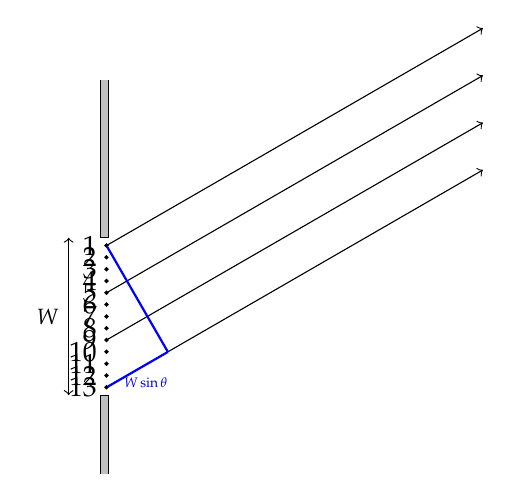
\begin{tikzpicture}
      \draw[fill=gray!50](0,3)--(0,1)--(-0.1,1)--(-0.1,3);
      \draw[fill=gray!50](0,-2)--(0,-1)--(-0.1,-1)--(-0.1,-2);
      \draw[<->](-0.5,-1)--(-0.5,1) node[midway,left]{\footnotesize $W$};
      \foreach \y in {1,...,13} {
        \pgfmathsetmacro\yy{1.05-0.15*\y};
        \draw[fill=black](-0.02,\yy) circle(0.02) node[left]{\Tiny\y};
        }
      \foreach \y in {1,5,9,13} {
        \pgfmathsetmacro\yy{1.05-0.15*\y};
        \draw[->,rotate around={30:(-0.02,\yy)}](-0.02,\yy)--(5.5,\yy);
      }

      \begin{scope}[rotate around={30:(-0.02,0.9)}]
        \draw[blue,thick](-0.02,0.88)--(-0.02,-0.66);
        \draw[blue,thick](-0.02,-0.66)--(-.9,-0.66)
        node[pos=.9,right]{\tiny $W\sin\theta$};
      \end{scope}
    \end{tikzpicture}

    \column{0.57\textwidth}
    \begin{itemize}
    \item Again, we follow what we did with the the previous case, and we
      find that at some angle $\theta$, the path difference between the top
      and bottom is $W\sin\theta=\frac{3}{2}\lambda$
    \item Beam from (1) and (5) differ by $\frac{\lambda}{2}$, so they
      have destructive interference; similarly 2 and 6, 3 and 7, 4 and 8,
      9 and 13 will all interfere destructively
    \item But some of the beams will not, so we have a bright fringe at the 
      projection
    \item This bright fringe is not as bright as the central one because
      of the destructive interference
    \end{itemize}
  \end{columns}
\end{frame}



\begin{frame}{Bright Fringes: Constructive Interference}
  Bright fringes exist on the screen at regular, half-numbered intervals
  ($m=1,2,3\ldots$):

  \eq{-.2in}{
    \boxed{\left(m+\frac{1}{2}\right)\lambda=W\sin\theta_m}
  }
  
  \vspace{-.1in}Again, similar to the dark fringes, we apply our small-angle
  approximation equation:

  \eq{-.2in}{
    \boxed{y_m=\left(m+\frac{1}{2}\right)\frac{\lambda L}{W}}
  }
\end{frame}



\begin{frame}{Single-Slit Diffraction, A Summary}
  \begin{itemize}
  \item Similar to the double-slit interference, single-slit diffraction
    projects a series of alternating bright fringes (``maxima'') and dark
    fringes (``minima'') in the far field
  \item The bright fringe in the middle (``central maximum'') is twice as wide
    and very bright
  \item Subsequent bright fringes on either side (``higher-order maxima'') are
    much dimmer because of the partial destructive interference
  \end{itemize}
  \begin{center}
    \pic{.65}{graphics/Single_Slit_Diffraction.png}
  \end{center}
\end{frame}



\section{Grating}

\begin{frame}{Diffraction Grating: What if there are more than 2 slits?}
  \begin{columns}
    \column{.35\textwidth}
    \pic{1.1}{graphics/grating1.png}
    
    \column{.66\textwidth}
    \begin{itemize}
    \item We can apply the same analysis from double-slit to a diffraction
      grating
    \item Use equation for double-slit interference to locate bright fringes
      
      \eq{-.2in}{
        n\lambda=d\sin\theta_n
      }
    \item Interference pattern is sharper
    \item Bright fringes are narrower
    \end{itemize}
  \end{columns}
\end{frame}



\section{Applications}

\begin{frame}{Optical Resolution}
  The ability of an optical instrument (e.g.\ the human eye, microscope,
  camera) to distinguish two distinct objects
  \begin{center}
    \pic{.322}{graphics/resolve1.png}\hspace{.05in}
    \pic{.322}{graphics/resolve2.png}\hspace{.05in}
    \pic{.322}{graphics/resolve3.png}\hspace{.05in}
  \end{center}
  When light from any object passes through an ``optical instrument'', it
  \textbf{diffracts}, therefore ``blurring'' the object
\end{frame}



\begin{frame}{Optical Resolution}
  \begin{columns}
    \column{.4\textwidth}
    \pic{1}{graphics/resolve4.png}

    \column{.6\textwidth}
    \textbf{Rayleigh limit}: Two objects are resolved if the angle
      $\theta>\theta_\mathrm{min}$, where $\theta_\mathrm{min}$ is when the first
      minimum (dark fringe) from object 1 overlaps with the central maximum
      (bright fringe in the middle) from object 2.
  \end{columns}
\end{frame}


\begin{frame}{Resolving Power}
  To resolve two objects, the minimum angle between rays from the two objects
  passing through an aperture is given by:
  $D$ of the aperture.
  \vspace{0.2in}
  \begin{columns}
    \column{0.5\textwidth}
    Rectangular aperture:

    \eq{-.2in}{
      \boxed{\theta_\mathrm{min}=\frac{\lambda}{W}}
    }
    \column{0.5\textwidth}
    Circular aperture:

    \eq{-.2in}{
      \boxed{\theta_\mathrm{min}=\frac{1.22\lambda}{D}}
    }
  \end{columns}
  where $W$ is the width of the aperture, and $D$ is the diameter of the
  aperture. The angle $\theta_\mathrm{min}$ is measured in \textbf{radians}.
\end{frame}



%\section[EM Wave]{Electromagnetic Wave}
%
%\begin{frame}
%  \frametitle{Maxwell's Equations}
%  \framesubtitle{We have already studied them}
%  
%  \vspace{-.3in}{\LARGE
%    \begin{align*}
%      \nabla\cdot\mb{E} &=\frac{\rho}{\varepsilon_0}\\
%      \nabla\cdot\mb{B} &= 0\\
%      \nabla\times\mb{E} &=-\frac{\partial\mb{B}}{\partial t}\\
%      \nabla\times\mb{B} &=-\mu_0\mb{J}+\mu_0\varepsilon_0\frac{\partial\mb{E}}{\partial t}
%    \end{align*}
%  }
%\end{frame}
%
%
%
%\begin{frame}
%  \frametitle{Maxwell's Equations}
%  \framesubtitle{Major Findings}
%  \begin{itemize}
%  \item Electric fields starts/ends at a charge
%  \item Magnetic fields runs in a loop, and has no beginning or ends
%  \item A changing electric field creates a magnetic field
%  \item A changing magnetic field creates an electric field
%  \item Disturbances in the electric and magnetic fields propagate as a wave
%    with speed
%    
%    \eq{-.2in}{
%      \boxed{c=\frac{1}{\sqrt{\varepsilon_o\mu_o}}=\SI{2.998e8}{m/s}}
%    }
%    \ldots the speed of light!
%  \end{itemize}
%\end{frame}
%
%
%
%\begin{frame}
%  \frametitle{Speed of Electromagnetic Radiation}
%  \begin{block}{Electric Permittivity $\varepsilon_0$}
%    The ability of a medium to resist the formation of an electric field within
%    it. The constant is directly related to the Coulomb constant in Coulomb's
%    law. 
%  \end{block}
%  \vspace{0.1in}
%  \begin{block}{Magnetic Permeability $\mu_o$}
%    A measure of the ability of the medium to become magnetized.
%  \end{block}
%
%  \begin{itemize}
%  \item Scientist have previously measured the speed of light to good accuracy
%  \item Maxwell's Equations show that light is (probably) an electromagnetic
%    (``EM'') wave
%  \item $\mb{E}$ and $\mb{B}$ fields of an EM wave are always perpendicular to
%    one another, according to Maxwell's Equations
%  \end{itemize}
%\end{frame}
%
%
%\begin{frame}
%  \frametitle{The Electromagnetic Spectrum}
%  \begin{center}
%    \pic{1}{graphics/electromagneticspectrum-141b490bac872789434.jpg}
%  \end{center}
%\end{frame}
%
%
%\begin{frame}
%  \frametitle{On Polarization of Light}
%  \framesubtitle{Let's Combine Everything We Know}
%  \begin{itemize}
%  \item Light is an electromagnetic wave, generated by
%    \begin{itemize}
%    \item An oscillating charged particle (e.g. shaking an electron violently)
%    \item An alternating (``A/C'') current (i.e.\ lots of oscillating charged
%      particles)
%    \item Through black-body radiation
%    \end{itemize}
%  \item The EM wave has both an oscillating electric field ($\mb{E}$) and
%    magnetic field ($\mb{B}$), because
%    \begin{itemize}
%    \item A charged particle creates an electric field, and
%    \item A moving charged particle creates a magnetic field
%    \end{itemize}
%  \end{itemize}
%\end{frame}
%
%
%\begin{frame}
%  \frametitle{On Polarizaion of Light}
%
%  A charged particle can vibrate in any direction, so the oscillating $\mb{E}$
%  and $\mb{B}$ can look quite chaotic. We can only guarantee that no matter
%  what happen, $\mb{E}$ and $\mb{B}$ are:
%  \begin{itemize}
%  \item Always perpendicular to each other
%  \item Always perpendicular to the direction of wave travel
%  \item This kind of light (or general EM wave) is ``unpolarized''
%  \item Most EM waves you experience in life are this kind
%  \end{itemize}
%  \begin{center}
%    \pic{0.7}{graphics/T1Zlt.png}
%  \end{center}
%\end{frame}
%
%
%\begin{frame}
%  \frametitle{On Polarization of Light}
%  But if we can confine $\mb{E}$ and $\mb{B}$ to one plane, then we have a
%  ``polarized'' light:
%  \begin{center}
%    \pic{0.4}{graphics/em-20field.jpg}
%  \end{center}
%  There are a few ways to do this\ldots
%\end{frame}
%
%\begin{frame}
%  \frametitle{On Polarization of Light}
%  \framesubtitle{Using Polarizer}
%  \begin{itemize}
%  \item A polarizer is really just a grill that only lets in vibration in one
%    direction through:
%    \begin{center}
%      \pic{0.45}{graphics/polarizerfencemodel600.jpg}
%    \end{center}
%  \item The incoming wave can be vibrating in any direction, but outgoing wave
%    only vibrates in one direction.
%  \item Sunglasses with polarizing lens
%  \item Polarizer filters on cameras
%  \end{itemize}
%\end{frame}
%
%\begin{frame}
%  \frametitle{On Polarization of Light}
%  \framesubtitle{Polarization by Reflection}
%  \begin{columns}
%    \column{0.4\textwidth}
%    \pic{1}{graphics/01fig16.jpg}
%    \column{0.57\textwidth}
%    At \textbf{Brewster's angle}, the light reflected off a medium (e.g.\
%    glass, water) is also polarized
%
%    \eq{-.1in}{
%      \theta_B =\tan^{-1}\left(\frac{n_2}{n_1}\right)
%    }
%    \begin{itemize}
%    \item Incident light is non-polarized
%    \item Reflected light is polarized
%    \item Refracted light is partially polarized
%    \item For water ($n=1.33$), $\theta_B=\ang{53}$
%    \item For glass ($n=1.5$), $\theta_B=\ang{56}$
%    \end{itemize}
%  \end{columns}
%\end{frame}
%
\end{document}
